\section{Gestore metodi d'accesso}
Il \textbf{gestore dei metodi di accesso}, per operare correttamente, deve conoscere una serie di informazioni fondamentali:

\begin{itemize}
	\item l'\textbf{organizzazione delle tuple all'interno dei blocchi};
	\item come sono \textbf{organizzati i blocchi al loro interno}.
\end{itemize}

In particolare, è necessario comprendere come è strutturata una \textbf{pagina} (o blocco) in memoria secondaria.
\begin{figure}[H]
	\centering
	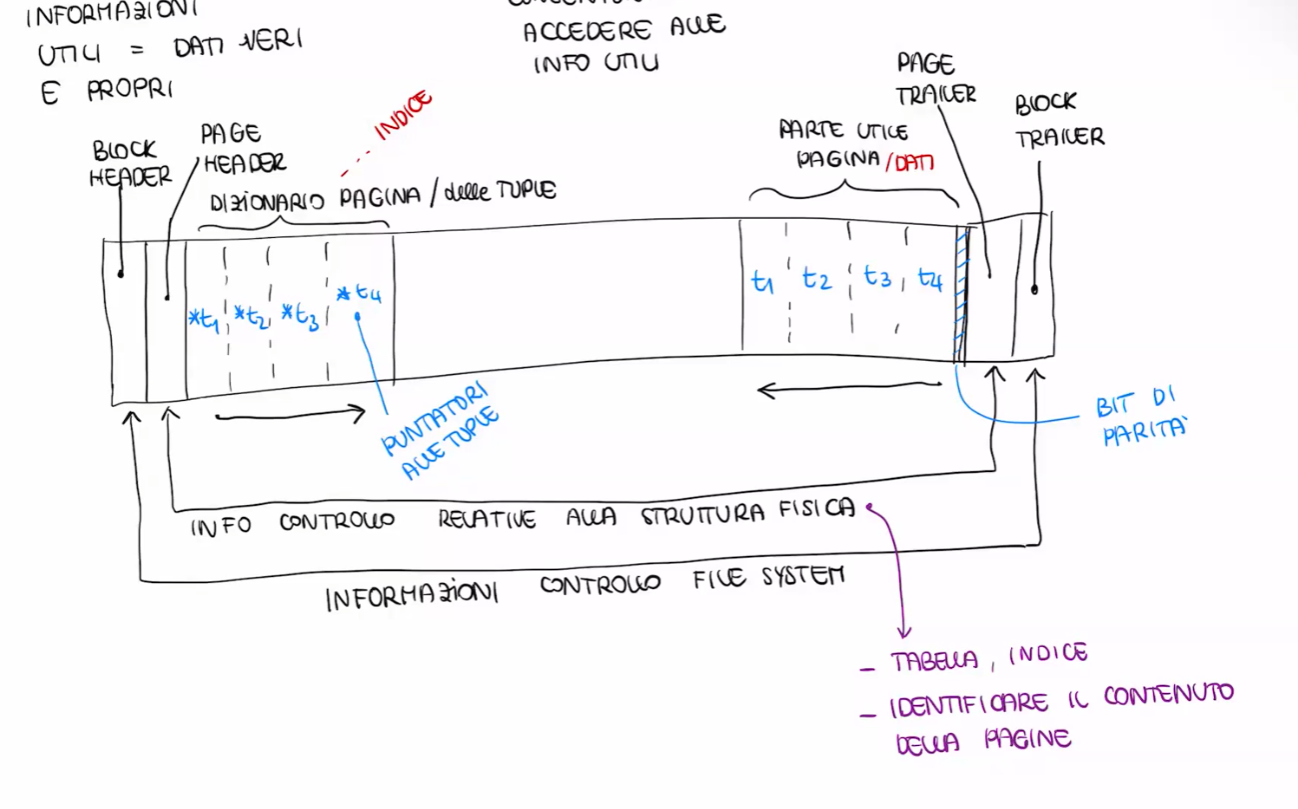
\includegraphics[width=1\linewidth]{image199}
	\caption{Struttura pagina}
	\label{fig:image199}
\end{figure}
Una pagina contiene due tipologie principali di informazioni:

\begin{itemize}
	\item \textbf{informazioni utili} (dati veri e propri), ovvero le tuple memorizzate;
	\item \textbf{informazioni di controllo}, che permettono di gestire e accedere correttamente ai dati.
\end{itemize}

Le informazioni di controllo sono fondamentali, poiché consentono al DBMS di localizzare, interpretare e manipolare i dati presenti nella pagina.

All'inizio e alla fine del blocco sono presenti strutture di controllo legate al file system:

\begin{itemize}
	\item \textbf{Block Header}: contiene informazioni di gestione del blocco;
	\item \textbf{Block Trailer}: contiene informazioni di controllo aggiuntive (ad esempio per verifiche di integrità).
\end{itemize}

Sono inoltre presenti informazioni di controllo relative alla \textbf{struttura fisica}, che permettono di:
\begin{itemize}
	\item identificare a quale tabella appartengono i dati;
	\item determinare se il blocco contiene dati o indici;
	\item interpretare correttamente il contenuto della pagina.
\end{itemize}

All'interno della pagina si distinguono due aree principali di memoria, che crescono in direzioni opposte:

\begin{itemize}
	\item il \textbf{dizionario della pagina} (o slot directory), che contiene puntatori alle tuple;
	\item la \textbf{parte utile della pagina}, che contiene effettivamente le tuple (dati).
\end{itemize}

Il dizionario della pagina può essere visto come una sorta di indice interno, che consente di accedere rapidamente alle tuple presenti nella pagina.

Un elemento importante è il \textbf{bit di parità}, utilizzato per verificare l'integrità dei dati e rilevare eventuali corruzioni delle informazioni.

Il dizionario delle tuple è necessario soprattutto quando le tuple hanno \textbf{lunghezza variabile}.

\begin{itemize}
	\item Nel caso di tuple a \textbf{lunghezza fissa}, non è necessario un dizionario, poiché la posizione delle tuple può essere calcolata direttamente.
	
	\item Tuttavia, questa soluzione è inefficiente, in quanto può causare \textbf{spreco di spazio}.
	
	\item Nel caso di tuple a \textbf{lunghezza variabile}, è invece necessario un dizionario, che memorizza per ogni tupla l'\textbf{offset di inizio} all'interno della pagina.
\end{itemize}

In questo modo, il DBMS può accedere direttamente alle tuple senza dover scansionare l'intero blocco, migliorando significativamente le prestazioni.
\subsection{Operazioni sulle pagine}

Il gestore dei metodi di accesso deve supportare diverse operazioni sulle pagine (blocchi), tra cui inserimento, cancellazione e accesso ai dati.

\subsubsection{Inserimento}

Nel caso di inserimento di una nuova tupla, si possono verificare tre situazioni:

\begin{itemize}
	\item \textbf{Spazio contiguo sufficiente} \\
	È il caso più semplice: la tupla viene inserita nella parte utile della pagina e il \textbf{dizionario della pagina} viene aggiornato con il nuovo puntatore (offset) alla tupla.
	
	\item \textbf{Spazio insufficiente} \\
	Se non esiste spazio sufficiente all'interno della pagina, è necessario interagire con il file system per allocare un \textbf{nuovo blocco}, nel quale verrà inserita la tupla.
	
	\item \textbf{Spazio sufficiente ma non contiguo} \\
	In questo caso è necessario effettuare una \textbf{riorganizzazione della pagina} (compattazione), in modo da rendere lo spazio libero contiguo. 
	Dopo la riorganizzazione, l'inserimento avviene come nel caso semplice.
\end{itemize}

\subsubsection{Cancellazione}

La cancellazione di una tupla è sempre possibile e generalmente non richiede una riorganizzazione immediata della pagina.

In particolare:
\begin{itemize}
	\item viene rimosso il riferimento alla tupla dal dizionario;
	\item lo spazio occupato dalla tupla viene marcato come libero.
\end{itemize}

Eventuali operazioni di compattazione possono essere eseguite in un secondo momento per ottimizzare lo spazio.

\subsubsection{Accesso}

L'accesso ai dati può avvenire in due modalità principali:

\begin{itemize}
	\item \textbf{Accesso a una tupla} \\
	Se è noto l'offset della tupla, si utilizza il \textbf{dizionario della pagina} per accedere direttamente alla posizione corretta. 
	In caso di accesso a più tuple, può essere conveniente effettuare una \textbf{scansione sequenziale} della pagina.
	
	\item \textbf{Accesso a un attributo} \\
	Per accedere a un attributo specifico, è necessario prima individuare la tupla. 
	Una volta identificata, si accede all'attributo tramite un meccanismo basato sugli \textbf{offset} interni alla tupla, che permettono di localizzare i singoli campi.
\end{itemize}
\subsection{Criteri di organizzazione delle tuple nei blocchi}

Le tuple all'interno dei blocchi possono essere organizzate secondo diversi criteri, in base a come vogliamo accedere ai dati.

Le principali modalità sono:

\begin{itemize}
	\item \textbf{Organizzazione sequenziale}: le tuple sono memorizzate una dopo l'altra, tipicamente nell'ordine di inserimento.
	
	\item \textbf{Accesso calcolato (hash)}: la posizione delle tuple è determinata da una funzione di hash, che permette un accesso diretto.
	
	\item \textbf{Strutture ad albero}: i dati sono organizzati tramite indici (es. B+-tree), per rendere più efficienti le ricerche.
\end{itemize}

\subsection{Organizzazione sequenziale dei file}

Consideriamo ora il caso più semplice: l'\textbf{organizzazione sequenziale}.

I dati sono salvati in file composti da blocchi logicamente consecutivi.  
Possiamo avere due varianti:

\begin{itemize}
	\item \textbf{Sequenziale disordinata (seriale)} → le tuple sono nell'ordine di inserimento
	\item \textbf{Sequenziale ordinata} → le tuple sono ordinate secondo una chiave
\end{itemize}

\subsubsection{Sequenziale disordinata (seriale)}

È la struttura più semplice e più intuitiva.

\paragraph{Inserimento}
L'inserimento è molto veloce:
\begin{itemize}
	\item si prende l'ultimo blocco del file;
	\item si inserisce la tupla lì dentro (se c'è spazio);
	\item si fa in genere un solo accesso al disco.
\end{itemize}

\paragraph{Ricerca}
La ricerca è il punto debole:
\begin{itemize}
	\item bisogna scorrere tutti i blocchi;
	\item quindi serve una scansione sequenziale;
	\item nel caso peggiore: $N$ accessi alla memoria secondaria.
\end{itemize}

\paragraph{Cancellazione}
\begin{itemize}
	\item prima bisogna trovare la tupla;
	\item poi si elimina;
	\item non si compatta subito lo spazio.
\end{itemize}

\paragraph{Modifica}
\begin{itemize}
	\item si trova la tupla;
	\item se cambia dimensione (tuple variabili), potrebbe non starci più;
	\item quindi si fa: cancellazione + inserimento.
\end{itemize}

\paragraph{Problema principale}

Queste operazioni (soprattutto cancellazioni e modifiche) creano \textbf{frammentazione} e spreco di spazio.

Per questo motivo il DBMS può eseguire delle \textbf{riorganizzazioni periodiche}, che servono a:
\begin{itemize}
	\item compattare i dati;
	\item recuperare spazio;
	\item migliorare le prestazioni.
\end{itemize}
\subsubsection{Sequenziale ordinata}

La \textbf{struttura sequenziale ordinata} è un file sequenziale in cui le tuple sono memorizzate in ordine rispetto a una \textbf{chiave di ordinamento}.

In generale, questa chiave può essere diversa dalla \textbf{chiave primaria} ed è scelta per ottimizzare determinate operazioni di accesso.

\paragraph{Caratteristiche principali}

\begin{itemize}
	\item le tuple sono mantenute \textbf{ordinate} secondo la chiave;
	\item i blocchi sono logicamente consecutivi;
	\item è possibile sfruttare l'ordinamento per rendere più efficienti le ricerche.
\end{itemize}
\begin{figure}[H]
	\centering
	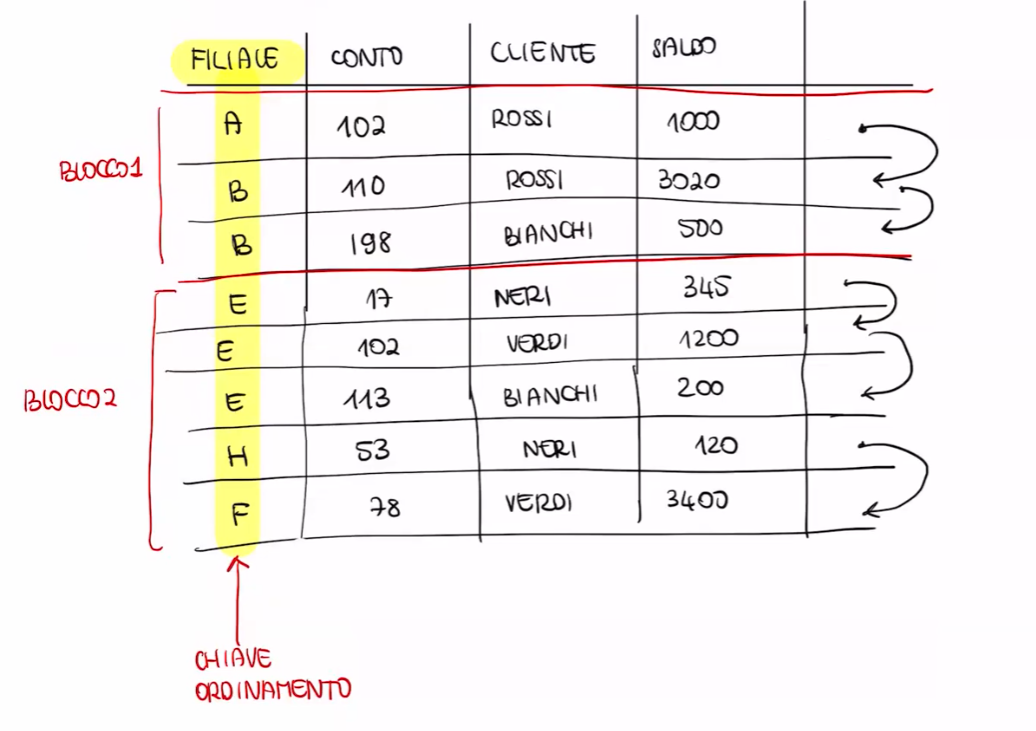
\includegraphics[width=0.75\linewidth]{image201}
	\caption{Esempio}
	\label{fig:image201}
\end{figure}
\begin{itemize}
	\item \textbf{Vantaggio} \\
	Rende efficienti tutte le operazioni che possono sfruttare l'\textbf{ordinamento}, 
	come ad esempio le ricerche per intervallo (es. ricerca per filiale).
	
	\item \textbf{Svantaggio} \\
	Le operazioni di aggiornamento (inserimento e modifica) devono mantenere l'ordinamento, 
	con un conseguente aumento del costo computazionale.
\end{itemize}